\let\negmedspace\undefined
\let\negthickspace\undefined
\documentclass[journal,12pt,twocolumn]{IEEEtran}
\usepackage{cite}
\usepackage{amsmath,amssymb,amsfonts,amsthm}
\usepackage{algorithmic}
\usepackage{graphicx}
\usepackage{textcomp}
\usepackage{xcolor}
\usepackage{txfonts}
\usepackage{listings}
\usepackage{enumitem}
\usepackage{mathtools}
\usepackage{gensymb}
\usepackage{comment}
\usepackage[breaklinks=true]{hyperref}
\usepackage{tkz-euclide}
\usepackage{listings}
\usepackage{gvv}                                        
\def\inputGnumericTable{}                                
\usepackage[latin1]{inputenc}                                
\usepackage{color}                                            
\usepackage{array}                                            
\usepackage{longtable}                                      
\usepackage{calc}                                            
\usepackage{multirow}                                        
\usepackage{hhline}                                          
\usepackage{ifthen}                                          
\usepackage{lscape}

\newtheorem{theorem}{Theorem}[section]
\newtheorem{problem}{Problem}
\newtheorem{proposition}{Proposition}[section]
\newtheorem{lemma}{Lemma}[section]
\newtheorem{corollary}[theorem]{Corollary}
\newtheorem{example}{Example}[section]
\newtheorem{definition}[problem]{Definition}
\newcommand{\BEQA}{\begin{eqnarray}}
\newcommand{\EEQA}{\end{eqnarray}}
\newcommand{\define}{\stackrel{\triangle}{=}}
\theoremstyle{remark}
\newtheorem{rem}{Remark}


\title{Assignment-2 SequenceAndSeries}
\author{Deepak Reddy ee23btech11047}
\date{January 2024}

\begin{document}

\maketitle
\section*{Exercise 9.1}
\textbf{Question:}\\
Write the first five terms of each of the sequences in Exercises 1 to 6 whose $n^{th}$
terms are:\\
4. $a_n = \frac{2n-3}{6}$\\
\textbf{Solution:}\\
$n^{th}$ term of the sequence is given by the above expression\\
we use n=1, we get First Term,
\begin{align}a_1 = \frac{2 \times 1 - 3}{6} = \frac{-1}{6} \end{align}\\
Similarly we will find other terms like this\\
we use n=2, we get Second Term,
\begin{align} a_{2} = \frac{2 \times 2 - 3}{6} = \frac{1}{6}  \end{align}\\
we use n=3, we get Third Term,
\begin{align} a_{3} = \frac{2 \times 3 - 3}{6} = \frac{1}{2} \end{align}\\
we use n=4, we get Fourth Term,
\begin{align} a_{4} = \frac{2 \times 4 - 3}{6} = \frac{5}{6} \end{align}\\
we use n=5, we get Fifth Term,
\begin{align} a_{5} = \frac{2 \times 5 - 3}{6} = \frac{7}{6} \end{align}\\
Therefore, The first five terms of the given sequence are
$a_1 = \frac{-1}{6}, a_2 = \frac{1}{6},a_3 = \frac{1}{2}, a_4 = \frac{5}{6},a_5 = \frac{7}{6}$\\
\\
\textbf{Question 2}\\
Express x(n) = $\frac{2n-3}{6}$ in terms of u(n) and find its Z transform\\
\textbf{Solution:}
The u(n) unit step function, which is defined as\\
$u(n) = 0$ if $ n < 0 $\\
$u(n)=1 $ if $n \ge 0 $\\
Now if we want to express x(n) in terms of u(n) we can break it into two parts: one for $n < 0 $ and one for $ n \ge 0$  
$$ x(n) = \frac{2n-3}{6} = \frac{n}{3} - \frac{1}{2} \cdot u(n) $$
Now if we want to find Z transform we can use
$$ X(Z) = \sum_{n = -\infty}^{\infty} x(n) \cdot Z^{-n}$$
Now we substitute
$x(n) = \frac{n}{3} - \frac{1}{2} \cdot u(n)$ in the above equation we get
$$ X(Z) = \sum_{n = 0}^{\infty} (\frac{n}{3} - \frac{1}{2} \cdot u(n) )\cdot Z^{-n} $$
Now we can write it as
$$ X(Z) = \sum_{n=0}^{\infty} \frac{n}{3} \cdot Z^{-n} - \sum_{n=0}^{\infty} \frac{1}{2} \cdot Z^{-n}$$
Now we will find the both summations
$$ \sum_{n=0}^{\infty} \frac{n}{3} \cdot Z^{-n} = \frac{1}{3} \cdot (0 + 1.Z^{-1} + 2.Z^{-2} + \ldots)$$
Now if we divide the above equation by $Z^{-1}$ we get
$$ Z^{-1} \cdot \sum_{n=0}^{\infty} \frac{n}{3} \cdot Z^{-n} =\frac{1}{3} \cdot (1.Z^{-2} + 2.Z^{-3} + \ldots )$$
Now if we subtract the above two equations we get
$$ \sum_{n=0}^{\infty} \frac{n}{3} \cdot Z^{-n} = \frac{Z}{Z-1} \cdot \frac{1}{3} \cdot (Z^{-1} + Z^{-2} + Z^{-3} + \ldots)$$

$$ \sum_{n=0}^{\infty} \frac{n}{3} \cdot Z^{-n} = \frac{1}{3} \cdot \left(\frac{Z}{(Z-1)^{2}}\right)$$
$$ \sum_{n=0}^{\infty} \frac{1}{2} \cdot Z^{-n} = \frac{1}{2} \cdot (1+Z^{-1} + Z^{-2} + \ldots) = \frac{1}{2} \cdot \frac{1}{1- Z^{-1}}$$
So now Z transform of the x(n) is
$$ X(Z) = \frac{1}{3} \cdot \frac{Z}{(Z-1)^{2}} - \frac{1}{2} \cdot \frac{1}{1-Z^{-1}}$$
$$X(Z) = {\frac{5Z-3 Z^{2}}{6(Z-1)^{2}}}$$
\newpage
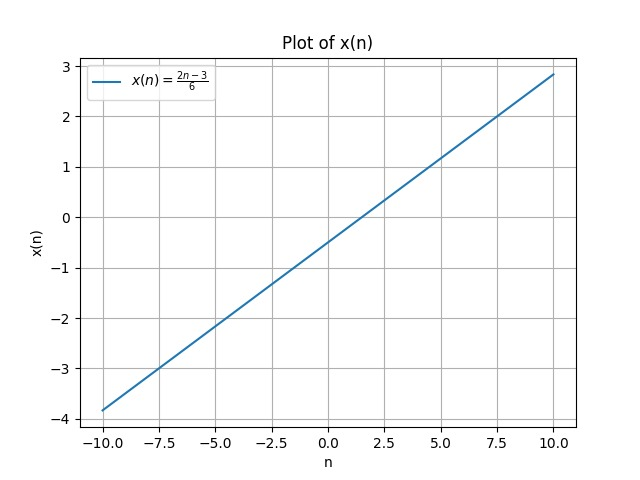
\includegraphics[width=0.55\textwidth]{graphgvv1.jpg}
\end{document}
